\documentclass[11pt]{article}

\usepackage[margin=1.1in]{geometry}
\usepackage{amsmath}
\usepackage{booktabs}
\usepackage{microtype}
\usepackage{tikz}
\usepackage[colorlinks=true,allcolors=blue]{hyperref}

\title{\textbf{Luce versus Thurstone on New Ground}\\[4pt]
\large\normalfont Choice-set restriction in large language models,\\
or why masking a logit is not removing an option}
\author{Peter Cotton}
\date{First version November 2024. This version 15 August 2026.}

\begin{document}
\maketitle

\begin{abstract}
\noindent A softmax renormalizes when a logit is masked, so it obeys Luce's
Choice Axiom for that operation. Restricting a choice set in language is a
different operation: the prompt changes and the logits are recomputed. We
measure which law describes the recomputation. Across thirteen designs and
48{,}536 cells, scored by exact log probabilities on all but one design,
Thurstonian contestant removal predicts restricted machine preference better
than renormalization, in all 99 question types of the original appendix and on
every model tested. The mechanism is mostly scale: restriction inflates
effective noise roughly fourfold, which renormalization cannot express and a
contest partly can. Granting each family one fitted scale shrinks the gap from
$0.140$ to $0.009$ nats, and a uniform rule over survivors beats both unfitted
defaults. What survives is a small, consistent advantage for the Gaussian shape
and a decisive one for abandoning renormalization. Explicit menus form a
separate regime violating every random utility model.
\end{abstract}

\section{Introduction}

Large language models can be interrogated cheaply and at scale, which makes
the study of their revealed preferences attractive whether one regards them
as incipient minds or as statistical mimics of our own predilections.
Either way, a question from the psychology of choice arises immediately:
when a model distributes probability over alternatives, what law governs
how that distribution changes as the set of alternatives changes?

The workhorse answer in economics and psychology is Luce's Choice Axiom
\cite{luce1959}, which asserts that the probability of selecting item $i$
from a set $S$ is proportional to a fixed utility $u(i)$:
\begin{equation}
P(i \mid S) = \frac{u(i)}{\sum_{j \in S} u(j)}.
\label{eq:luce}
\end{equation}
Its signature is Independence of Irrelevant Alternatives: the ratio
$P(A)/P(B)$ is unchanged by the presence or absence of a third option $C$.

There is a natural alignment between this assumption and the token
probabilities of language models, which invariably emerge from a softmax:
\begin{equation}
p_i = \frac{e^{z_i}}{\sum_{j=1}^n e^{z_j}},
\label{eq:softmax}
\end{equation}
however complicated the transformer computation producing $z_i$ may be.
Delete item 1 by setting $z_1 = -\infty$, a surgical procedure impossible in
humans, and the remaining probabilities are the old ones renormalized by
$1/(1-p_1)$. The output layer therefore satisfies the Choice Axiom exactly,
for that operation.

Restricting a choice set in language is not that operation, and we do not
suppose it is. Telling a model that an option is unavailable changes the
prompt, so the whole logit vector is recomputed rather than masked, and
nothing in the architecture constrains the new odds among survivors to match
the old ones. Menu-dependent logits can represent any positive choice rule at
all. The softmax is thus a statement about what the sampling head does with a
\emph{fixed} state, not a prediction about behaviour across prompts, and the
question of which law describes the recomputation is empirical from the
outset.

That gap is the subject of this paper, and it has practical bite because
masked renormalization is exactly what deployed systems compute: constrained
decoding, tool routers that mask unavailable tools, and guardrails that drop
a candidate all impose Equation~\eqref{eq:luce} by construction. What a model
reports when told in context that an option is unavailable is a different
object. We measure how far apart the two are, and find the difference better
described by the Thurstonian contest of \cite{thurstone1927} than by
renormalization.

The evidence is not a single experiment. Table~\ref{tab:designs} lists
thirteen designs comprising $73{,}704$ scored choice cells, built from
$61{,}512$ logged exact log-probability measurements on five commercial and
fourteen open-weight models, alongside the masked language model study of the 2024 version and a
generative replication on Claude. Every cell is a zero-parameter
out-of-sample prediction: both families are calibrated to an unrestricted
distribution and asked to predict a restricted one they have not seen. The
two largest batteries, $3{,}660$ and $1{,}195$ cells, favor the contest
model with bootstrap confidence intervals excluding zero on every one of
the five models, and the margin rises monotonically with model tier, from
$+0.30$ on GPT-4.1-nano to $+0.88$ on GPT-4.1. All raw model responses are
logged and released, so every number below is recomputable without further
inference.

Section~\ref{sec:models} states the two competing models and
Section~\ref{sec:history} places the comparison in the century of
psychometric and econometric argument it belongs to.
Sections~\ref{sec:masked}--\ref{sec:maskedresults} test them on masked
language models. Section~\ref{sec:polysemy} moves to modern models under
exact measurement, using polysemous words as the entry probe and
connecting the paradox to the stated-versus-generated gap recently
documented by Cekinmez, Wu, Marjieh and Griffiths \cite{cekinmez2026}.
Section~\ref{sec:discussion} draws out the implications, and separates what the
measurements support from three conjectures they merely motivate: a mechanism
for generative ``mode collapse'', a diversity knob, and a contest-structured
output layer.

\begin{table}[ht]
\centering
\small
\begin{tabular}{llrl}
\toprule
Design & Models & Cells & Verdict \\
\midrule
Adjective qualification (masked) & 2 masked LMs & 100+ & Thurstone $\approx 80\%$ \\
Two-slot elimination (masked) & 2 masked LMs & 100+ & Thurstone $\approx 80\%$ \\
Polysemous generation, restriction & Claude & 21 & re-collapse, not renormalization \\
Qualified-noun restriction & 3 GPT & 71 & tie (degenerate priors) \\
Random elicitation, one deletion & 3 GPT & 77 & Thurstone 39/56, $p = 0.002$ \\
Permutation-controlled deletion & 5 GPT & 1{,}195 & $+0.025$ $[+0.009, +0.047]$ \\
Original 2024 stimuli, two-slot & 5 GPT & 3{,}660 & $+0.519$ $[+0.443, +0.600]$ \\
Open-vocabulary sweep, 99 question types & 3 GPT & 37{,}764 & \textbf{99/99 types favor Thurstone} \\
\quad pooled estimate & & & $+0.150$ $[+0.135, +0.165]$ \\
Ordered selection to depth five & 5 GPT & 1{,}363 & $+0.339$ $[+0.248, +0.438]$ \\
Reversibility (best vs worst first) & 5 GPT & 108 & $-0.290$ $[-1.060, +0.425]$; neither family \\
Block--Marschak / RUM test & 5 GPT & 30 & 30/30 violate RUM \\
Menu deletion under conditioning & 5 GPT & 229 & $+0.026$ $[+0.008, +0.045]$ \\
Duplicates, decoys, compromise & 5 GPT & 101 & substitution 15/41; regularity 23/60 \\
Local panel on the same stimuli & 14 open & 24{,}948 & tuning effect in 4 of 6 pairs \\
Local inventory panel & 14 open & 4{,}158 & $+0.015$ $[+0.012, +0.018]$ \\
\bottomrule
\end{tabular}
\caption{The full evidence base, recomputed from the released logs. Cells are
scored zero-parameter predictions of a restricted distribution, and intervals
are cluster bootstraps over the design's natural grouping (question type,
category or family) rather than over cells. Every design but the polysemy
replication uses exact log probabilities. Masked language model counts are
category/adjective combinations from the 2024 version.}
\label{tab:designs}
\end{table}


\begin{figure}[t]
\centering
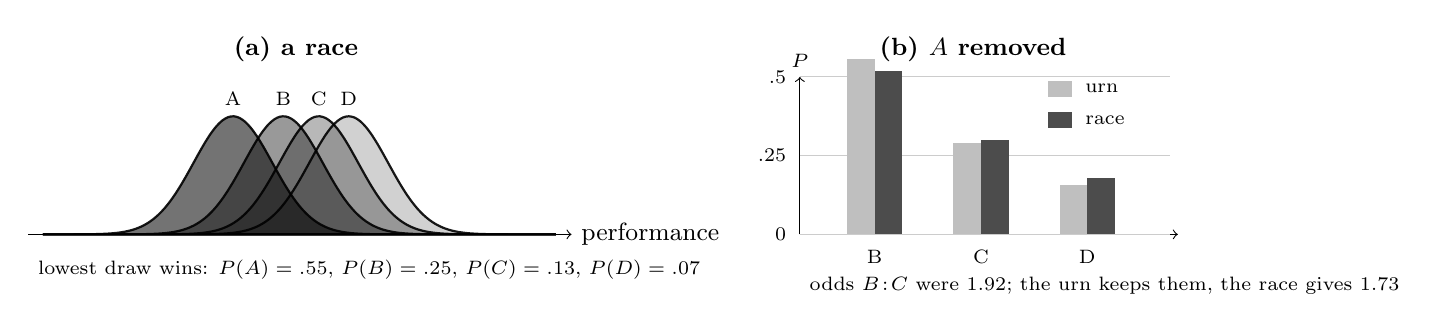
\begin{tikzpicture}[scale=1.0]
% ---- panel (a): the race ----
\begin{scope}
  \draw[->] (-3.4,0) -- (3.5,0) node[right] {\small performance};
  \foreach \mu/\lab/\pw/\sh in {-0.80/A/.55/0.55, -0.16/B/.25/0.40,
                                0.29/C/.13/0.28, 0.67/D/.07/0.18} {
    \draw[thick, fill=black, fill opacity=\sh, draw opacity=0.9]
      plot[domain=-3.2:3.3, samples=90, smooth]
      (\x, {1.5*exp(-(\x-\mu)*(\x-\mu)/0.5)}) -- (3.3,0) -- (-3.2,0) -- cycle;
    \node[font=\scriptsize] at (\mu, {1.5*exp(0)+0.22}) {\lab};
  }
  \node[font=\scriptsize, anchor=west] at (-3.4,-0.45)
    {lowest draw wins: $P(A)=.55$, $P(B)=.25$, $P(C)=.13$, $P(D)=.07$};
  \node[font=\small\bfseries] at (0,2.35) {(a) a race};
\end{scope}
% ---- panel (b): A removed ----
\begin{scope}[xshift=8.6cm]
  \node[font=\small\bfseries] at (0,2.35) {(b) $A$ removed};
  \draw[->] (-2.2,0) -- (2.6,0);
  \draw[->] (-2.2,0) -- (-2.2,2.0) node[above, font=\scriptsize] {$P$};
  \foreach \y/\lab in {0/0, 1.0/.25, 2.0/.5} {
    \draw[gray!40] (-2.2,\y) -- (2.5,\y);
    \node[font=\scriptsize, anchor=east] at (-2.25,\y) {\lab};
  }
  % Luce (renormalized) and Thurstone (re-raced) bars
  \foreach \i/\lab/\lu/\th in {0/B/2.222/2.080, 1/C/1.156/1.203, 2/D/0.622/0.717} {
    \fill[black!25] ({-1.6+\i*1.35},0) rectangle ({-1.25+\i*1.35},\lu);
    \fill[black!70] ({-1.25+\i*1.35},0) rectangle ({-0.90+\i*1.35},\th);
    \node[font=\scriptsize] at ({-1.25+\i*1.35},-0.28) {\lab};
  }
  \fill[black!25] (0.95,1.75) rectangle (1.25,1.95);
  \node[font=\scriptsize, anchor=west] at (1.3,1.85) {urn};
  \fill[black!70] (0.95,1.35) rectangle (1.25,1.55);
  \node[font=\scriptsize, anchor=west] at (1.3,1.45) {race};
  \node[font=\scriptsize, anchor=west] at (-2.2,-0.65)
    {odds $B\!:\!C$ were $1.92$; the urn keeps them, the race gives $1.73$};
\end{scope}
\end{tikzpicture}
\caption{The two models disagree only under restriction. In (a) each item
draws a performance and the lowest wins, which for these locations gives the
win probabilities shown. In (b) item $A$ is removed. The urn rescales what is
left, so the odds between any two survivors are unchanged by construction. The
race is re-run without $A$, and the mass it vacated is redistributed unevenly:
$B$ gains less than proportionally and the tail gains more, moving the $B\!:\!C$
odds from $1.92$ to $1.73$. Every battery in this paper measures which of these
two reallocations a language model performs. Locations are calibrated to the
win probabilities in (a) by the method of \cite{cotton2021}; the numbers are
exact, not illustrative.}
\label{fig:urnrace}
\end{figure}

\section{A choice of choice models}
\label{sec:models}

One might describe Equation~\eqref{eq:luce} as an \emph{urn model}: item
$k$ is represented by balls in an urn in proportion to $u(k)$, a choice is
a random draw, and shrinking the choice set merely removes balls. The
renormalization of probability under restriction then seems perfectly
reasonable.

But perhaps preference is a horse race, not an urn. In the competing model
each item $i$ carries a location parameter $a_i$ (a dislikability, say) and
an associated performance $X_i \sim N(a_i, 1)$. Item $i$ is chosen when its
performance is the lowest draw. This is the model of Thurstone
\cite{thurstone1927}, and it makes different predictions about how choice
probabilities respond when the choice set is altered: rather than removing
a ball from the urn, we remove a horse from the race.

Unit variance and independence make this Case V, the family's default and its
tightest special case. Everything below uses it, and Section~\ref{sec:tilt}
explains why: richer contests would fit better, but Luce in its bare form has
nothing to fit, so comparing a searched Thurstone against an unsearched Luce
would prove little.

(As an aside, it \emph{is} possible to engineer a contest that satisfies
Luce's Choice Axiom, by taking $X_i \sim \mathrm{Exp}(h_i)$ with common
location and differing hazard rates, or, by Yellott's theorem, with
Gumbel noise \cite{yellott1977}. The comparison here can therefore be
viewed as between two noise families within the contest framework, which
is why single-menu fits cannot separate them and the restriction,
duplication, and context designs below are required.)

The practical obstacle to Thurstonian models has always been computation,
not plausibility. A fast lattice algorithm for calibrating multi-entrant
Thurstone models, recovering locations $\{a_i\}$ from winning
probabilities and computing derived quantities for fields exceeding
$100{,}000$ entrants, was given in \cite{cotton2021}, and is what makes
the experiments below routine.

\subsection{A hundred years of the same argument}
\label{sec:history}

The question this paper puts to language models is not a new one. It has
been contested continuously since Thurstone published the law of comparative
judgment in 1927 \cite{thurstone1927}, building on Fechner's discriminal
dispersions \cite{fechner1860}, and it has never been settled in either
direction.

The interesting historical question is not who was right but why one side won,
because it did not win on the evidence. It won on arithmetic.

Thurstone's contest has no closed form beyond two alternatives. Choosing among
$n$ items requires the probability that one normal draw is extremal among $n$,
an $(n-1)$-dimensional integral with no elementary expression. Case V, the
equal-variance independent case that Mosteller \cite{mosteller1951} made
usable, reduces the \emph{paired} comparison to $\Phi(d/\sqrt{2})$ and no
further. Everything past a pair needed numerical integration on machinery that
did not exist, and when the econometric version was finally written down as
multinomial probit \cite{hausman1978} it was reported as practical only for a
handful of alternatives. Simulation methods made it estimable in the 1990s and
it remains the expensive option \cite{train2009}.

The logistic alternative had the opposite property. Bradley and Terry
\cite{bradley1952} wrote a paired comparison model with a closed form, a
concave log-likelihood and estimation by hand. Luce \cite{luce1959} then
supplied the axiom, deriving Equation~\eqref{eq:luce} from Independence of
Irrelevant Alternatives, which converted a computational convenience into a
behavioral principle: the form was no longer merely tractable, it was
\emph{implied} by a plausible-sounding condition on choice. McFadden
\cite{mcfadden1974} made it the workhorse of applied discrete choice, and
Yellott \cite{yellott1977} completed the retrospective justification by
showing exactly which noise distribution the axiom corresponds to, which had
the side effect of making the double exponential look canonical rather than
merely convenient.

The pattern of the century that followed is that the Luce form was repaired
rather than replaced. Nested logit, the generalized extreme value family and
mixed logit \cite{mcfaddentrain2000} were all built to relax the independence
IIA imposes while keeping the closed form that made the logit estimable.
Choosing the Thurstonian route instead would have meant paying the integral,
and almost nobody did.

The objections were immediate and they were about restriction. Debreu
\cite{debreu1960}, reviewing Luce's book, observed that adding a near
duplicate of an existing alternative should divide that alternative's share
rather than draw proportionally from everything, which IIA cannot do. Tversky
\cite{tversky1972} showed that similarity between alternatives violates
simple scalability altogether and proposed elimination by aspects instead.
Luce \cite{luce1977} himself reviewed the axiom's standing after twenty
years and treated its empirical failures as established rather than
contested. In econometrics the same problem drove a long sequence of
repairs: McFadden's conditional logit \cite{mcfadden1974} made the Luce form
the workhorse of discrete choice, then nested logit, the generalized extreme
value family and mixed logit \cite{mcfaddentrain2000} were built to relax
the independence it imposes, with Hausman and McFadden
\cite{hausman1984} providing a specification test for the violation.

Two results from that literature bear directly on what follows. Yellott
\cite{yellott1977} proved that Luce's axiom holds in a random utility
contest if and only if the noise is double exponential, which places the two
families inside one framework and identifies the disagreement as a question
about noise rather than about utility. Block and Marschak
\cite{block1960} and Falmagne \cite{falmagne1978} characterized when a
complete choice structure admits any random utility representation at all, by
nonnegativity of the Block--Marschak polynomials, which supplies a test that
does not presuppose either family. Section~\ref{sec:menus} applies it.

The dispute also has a quantitative history outside psychology. In racing
markets, Harville's renormalization \cite{harville1973} is the Luce
prediction applied to finishing order, and its systematic mispricing of
second and third place is well documented; Henery \cite{henery1981} and
Stern \cite{stern1990} proposed normal, that is Thurstonian, order models to
correct it, and the correction works. The two-slot design of
Section~\ref{sec:masked} is that comparison transplanted into a language
model.

Two things have changed, and together they are why the question is worth
reopening now rather than in 1977. The integral is no longer expensive: the
lattice method of \cite{cotton2021} returns the whole vector of winning
probabilities for fields of $10^5$ entrants, so the tractability argument that
decided the matter has expired. And the measurement is no longer noisy. A
century of this dispute was conducted on human subjects, where a choice
distribution must be estimated from repeated trials and the standard errors
swamp the difference between the two families on any single menu. A language
model reports its distribution directly, to as many digits as one wants, which
turns a question that needed thousands of participants into one that needs a
few thousand API calls.

What makes the machine case worth revisiting is also that one side of this
argument has been built into the apparatus. A softmax output layer is the
Luce form, so an LLM's sampling head satisfies the Choice Axiom by
construction. Reward models for preference tuning are Bradley--Terry
\cite{bradley1952}, fitted to pairwise human comparisons on the assumption
that a single scalar utility governs choice, and Direct Preference
Optimization \cite{rafailov2023} inherits the same likelihood. Listwise
ranking objectives use Plackett--Luce \cite{plackett1975}. The modern
pipeline therefore assumes the Luce side of a century-old and unresolved
dispute at three separate points, which makes the question of whether the
resulting behavior obeys the axiom an empirical matter with some
consequence, and one that exact log probabilities can settle in a way that
human subjects never could.

\section{Experimental design: masked language models}
\label{sec:masked}

We probe the token probabilities of BERT \cite{devlin2018} and RoBERTa
\cite{liu2019}, prompted to fill in blanks that invite choices among items
of a category. Two designs are used.

In the first, the model answers an \emph{original} question and a
\emph{qualified} question whose only difference is an adjective that
shrinks the choice set:
\begin{enumerate}
\item \emph{Original:} ``My favorite state in the U.S. is [MASK] and I try
to visit once a year.''
\item \emph{Qualified:} ``My favorite Western state in the U.S. is [MASK]
and I try to visit once a year.''
\end{enumerate}
\footnote{No qualifier partitions a category cleanly. Some Western states are
more western than others, Oklahoma and Texas being the obvious hard cases,
and a reader who disagrees with any particular assignment is probably right.
The same fuzziness attends every design here: senses of a polysemous word
overlap, ``a random $X$'' is not a uniform draw, a two-slot continuation
invites contrast and collocation as well as exclusion, and an adjective alters
what the question means as well as which answers remain admissible. So none of
these manipulations is a surgical deletion from a fixed choice problem, and
machine restriction is not a pure urn problem in any case. What the designs
require is weaker: that the manipulation removes an item from serious
contention, and that both candidate laws face the identical stimulus. A
qualifier whose boundary is arguable adds noise to the comparison rather than
favouring either family, and the batteries are large enough, and the
restriction phrasings varied enough, that no single fuzzy boundary carries the
result. The exclusion phrasing of Section~\ref{sec:sweep} is the cleanest
instrument, and it is reported separately throughout.}

In the second, we eliminate a single option explicitly, feeding the top
answer of a first prompt back into a second:
\begin{enumerate}
\item \emph{First:} ``My favorite primary color is [MASK] because it is
SOMETHING.''
\item \emph{Second:} ``My two favorite primary colors are [ANSWER] and
[MASK] because they are SOMETHING.''
\end{enumerate}
where SOMETHING ranges over many adjectives so that luck of phrasing is
averaged out (the appendix of the working version lists roughly one
hundred category/adjective combinations).

Both models make zero-parameter predictions of the restricted
distribution from the unrestricted one. Luce's prediction is
renormalization, Equation~\eqref{eq:luce}; in the two-step design this is
the simplest Plackett--Luce \cite{plackett1975} or Harville
\cite{harville1973} construction. The Thurstonian prediction calibrates
locations $\{a_i\}$ to the unrestricted token probabilities via
$\mathrm{Prob}(X_i < X_k \;\forall k \neq i) = p_i$, removes the excluded
contestant, and recomputes winning probabilities.

\section{Results for masked language models}
\label{sec:maskedresults}

Table~\ref{tab:western} shows the ``favorite Western state'' prompt for
BERT. The Thurstonian column tracks the actual restricted probabilities
more closely than Luce renormalization, which overweights the favorite
(California) at the expense of the field. Table~\ref{tab:names} repeats
the exercise for ``favorite girl's baby name'', where the RMSE using
Luce's probabilities is roughly 50\% higher.

\begin{table}[ht]
\centering
\begin{tabular}{lrrrr}
\toprule
State & Original (\%) & Luce (\%) & Thurstonian (\%) & Actual (\%) \\
\midrule
California & 10.89 & 29.87 & 25.38 & 20.17 \\
Arizona    &  6.74 & 18.50 & 17.20 & 10.00 \\
Texas      &  5.50 & 15.10 & 14.59 &  7.68 \\
Colorado   &  3.18 &  8.74 &  9.38 &  7.81 \\
Oregon     &  2.89 &  7.92 &  8.67 &  8.57 \\
Oklahoma   &  1.97 &  5.41 &  6.37 &  6.64 \\
Nevada     &  1.66 &  4.55 &  5.54 & 10.18 \\
Montana    &  1.59 &  4.37 &  5.36 & 14.27 \\
Idaho      &  1.05 &  2.87 &  3.82 &  4.99 \\
Wyoming    &  0.98 &  2.69 &  3.62 &  9.69 \\
\bottomrule
\end{tabular}
\caption{Predicted probabilities under Luce's Choice Axiom and the
Thurstonian model for the ``favorite Western state'' prompt
(BertForMaskedLM). Both predictions use only the unqualified token
probabilities; the Thurstonian model is closer to the actual qualified
probabilities.}
\label{tab:western}
\end{table}

\begin{table}[ht]
\centering
\begin{tabular}{lrrrr}
\toprule
Name & Original (\%) & Luce (\%) & Thurstonian (\%) & Actual (\%) \\
\midrule
Lily     & 1.56 & 20.35 & 16.18 & 14.52 \\
Emily    & 1.15 & 15.06 & 13.31 & 16.29 \\
Mia      & 0.86 & 11.25 & 11.02 & 13.18 \\
Bella    & 0.85 & 11.12 & 10.93 &  8.84 \\
Sarah    & 0.68 &  8.89 &  9.44 &  9.41 \\
Rachel   & 0.59 &  7.66 &  8.56 &  7.15 \\
Kate     & 0.59 &  7.63 &  8.54 &  8.44 \\
Lauren   & 0.47 &  6.11 &  7.39 &  7.23 \\
Brittany & 0.46 &  6.04 &  7.33 &  7.55 \\
Chloe    & 0.45 &  5.89 &  7.21 &  7.39 \\
\bottomrule
\end{tabular}
\caption{The same comparison for ``favorite girl's baby name''. The RMSE
using Luce's probabilities is approximately 50\% higher than the
Thurstonian RMSE.}
\label{tab:names}
\end{table}

Across the full panel of qualified-question and single-item-elimination
experiments, the Thurstonian model provides the more accurate prediction
in approximately 80\% of cases, with its advantage concentrated where the
qualification is substantial and the entropy of the unrestricted
distribution is low.
% Figures 1 and 2 of the July 2024 version (entropy scatter; per-category
% RMSE bars) belong here; source files live with the original draft.

\section{Modern models under exact measurement}
\label{sec:polysemy}

Cekinmez, Wu, Marjieh and Griffiths \cite{cekinmez2026} recently turned an
everyday property of language into a measurable distribution over
meanings: give a model a bare polysemous word (``bolt'') with no
disambiguating context, sample many outputs, and classify which sense each
expresses. Across 32 text and image generation models they report a
striking ladder of normalized sense entropies: image generation $0.10$,
text generation $0.25$, human subjects $0.47$, and, when models are asked
to \emph{predict} the distribution of senses, roughly $0.73$. Models
know the ambiguity; they do not express it. The finding sits within a
growing literature on generative homogenization \cite{jiang2026} and its
sharpening under preference tuning \cite{kirk2024}; their own ablation
shows DPO alone cutting sense entropy from $0.25$ to $0.18$.

Read through the lens of Section~\ref{sec:models}, the ladder is what a
contest model produces. Let the stated distribution proxy the latent
locations $\{a_i\}$; let each generation be a contest among noisy sense
performances. When noise is small relative to the spread of locations, winning probability
is a steeply nonlinear function of location differences, sigmoidal rather than
convex, and a mildly uneven prior collapses onto its mode. One noise
parameter then indexes the entire ladder, and the ``multimodal gap''
becomes a noise gap rather than a knowledge gap. The rival explanation is
a power tilt: renormalized $p_i^{\gamma}$, the Luce family with a
temperature. Low-temperature decoding is literally this transformation of a
fixed token distribution. Preference tuning and classifier-free guidance are
often described in the same terms but are not the same operation: tuning
changes parameters, and therefore logits, in a prompt- and token-dependent
way, while guidance combines conditional and unconditional logits. The tilt is
a rival account of the observed sharpening, not a description of what those
procedures compute. The two families are
distinguished not by the collapse itself but by behavior under choice-set
restriction, precisely the instrument of Section~\ref{sec:masked}, and an
experiment run by neither paper until now.

\subsection{Replication on a chat model}

The smallest of our designs, and the only one using sampling rather than
exact probabilities, replicates their generative setup on Claude models
(October 2025 generation): 15 polysemous words from the stimulus set of
\cite{cekinmez2026}, 150 independent sentence generations per word, senses
classified by a second model against the closed inventory, plus a stated
distribution elicited with their ``predicting itself'' framing. The
collapse replicates almost exactly: mean normalized sense entropy $0.252$
generated (their text-model figure: $0.25$) against $0.880$ stated.

Fitting the two one-parameter families from stated to generated
distributions gives a statistical tie (Thurstone $\sigma = 0.42$, RMSE
$0.273$; power tilt $\gamma = 2.25$, RMSE $0.273$; Thurstone the better
fit on 10 of 15 words), and the reason both fit poorly is itself
informative: for several words the generated mode is not even the stated
argmax (``port'' generates \emph{harbor} in every sample while rating
\emph{connector} most probable). Stated reports are a biased window on
the latent locations, not merely a flattened one. This is consistent with
\cite{cekinmez2026}, whose stated distributions overestimate even human
diversity. Calibration should therefore use revealed behavior, which is
what the restriction design does.

\subsection{Choice-set restriction}

For the six words whose unrestricted distributions were non-degenerate,
we re-sampled with the modal sense excluded by instruction (150 samples
per condition) and compared zero-parameter predictions of the restricted
distribution: Luce renormalization against Thurstonian contestant
removal, both calibrated to the add-half smoothed unrestricted sense
counts.

\begin{table}[ht]
\centering
\begin{tabular}{lrrl}
\toprule
Word & Luce RMSE & Thurstonian RMSE & Restricted distribution \\
\midrule
bolt  & 0.450 & \textbf{0.413} & fastener .68, run .18, lock .14 \\
seal  & \textbf{0.077} & 0.089 & animal .67, close .33 \\
pitch & 0.655 & \textbf{0.630} & throw .06, tone .31, field .63 \\
bat   & 0.559 & \textbf{0.546} & animal 1.00, hit .00 \\
match & 0.758 & \textbf{0.651} & firestick .82, contest .18 \\
iron  & \textbf{0.002} & 0.037 & metal .95, press .04, golf .01 \\
\midrule
pooled & 0.495 & \textbf{0.459} & \\
\bottomrule
\end{tabular}
\caption{Restriction test on polysemous words (Claude Haiku 4.5, 150
samples per condition, modal sense excluded by instruction). The
Thurstonian prediction is closer pooled and on four of six words
(bootstrap over words: $P(\text{Thurstone better}) = 0.90$).}
\label{tab:restrict}
\end{table}

The margin favors Thurstone, but the qualitative signature matters more
than the margin: under restriction the model does not spread probability
proportionally, as Luce requires. It \emph{re-collapses} onto a new modal
sense (match $\to$ \emph{firestick} at $.82$; iron $\to$ \emph{metal} at
$.95$; bat $\to$ \emph{animal} at $1.00$). Remove the winning horse and
the runner-up now wins nearly always. That is low-noise contest behavior,
in the same low-entropy, heavy-qualification regime where the Thurstonian
advantage concentrated in Section~\ref{sec:maskedresults}. Some rank
flips under restriction exceed even the Thurstonian sharpening, and
inventories with overlapping senses (``bat'') contaminate the exclusion
instruction; neither family survives those cells.

\subsection{Exact probabilities on GPT models}

Sampling noise can be removed entirely on models that expose token log
probabilities. We ported the qualified-question design of
Section~\ref{sec:masked} to GPT-4o-mini, GPT-4o and GPT-4.1: twenty
category pairs (``my favorite color is'' / ``my favorite warm color
is''), two phrasings, next-token distributions read exactly from the
top-20 log probabilities, with the Thurstonian field restricted to a
declared category inventory. Across 71 usable cells the comparison is a
statistical tie with a Thurstonian lean: Thurstone wins 38 of 71 cells
and has the lower pooled RMSE on all three models (e.g.\ $0.290$ vs
$0.295$ on GPT-4o), but a bootstrap over cells does not separate the
families ($p = 0.29$).

The instrument, however, has weakened for an interesting reason: the
unqualified distributions of preference-tuned chat models are already
near-degenerate (``my favorite tree is'' puts $0.94$ on \emph{oak}),
so most cells carry little discriminating information. Under either
model the surviving favorite keeps nearly everything, and the comparison
hinges on tail probabilities. The masked models of
Section~\ref{sec:maskedresults} answered the unqualified question with
entropy to spare (California at $10.9\%$); their preference-tuned
descendants have already collapsed before the experimenter arrives. This
is the same collapse measured by \cite{cekinmez2026}, now visible as a
loss of experimental power: alignment has pushed the interesting
variation into the tails, where only exact log-probability designs can
reach it.

\subsection{Random elicitation restores the regime}

The remedy is to ask for randomness rather than preference. ``Name a
random programming language'' followed by explicit single-item
elimination raises mean unqualified entropy to $0.38$ and returns the
experiment to the regime where the two families disagree. The elimination
takes one of two forms, either an exclusion (``\ldots{} that is not
Python'') or the two-slot continuation of Section~\ref{sec:masked} (``I
already picked one random programming language: Python. Name
another\ldots''). The recovery is only partial, since
models are poor samplers even on request, with ``a random planet''
putting essentially all mass on \emph{Mars}. The homogenization of
\cite{jiang2026} extends to explicit randomness.

To control for phrasing and for which item is removed, the definitive
battery deletes \emph{each} of the top eight observed items in turn,
under two phrasings, across 50 categories and three GPT models. Thirty-one
categories retain enough inventory-matched mass to be scorable, giving 692
permutation-controlled cells on the three headline models and 1{,}195 once the
two cheaper models are added, scored by the proper rule $\mathrm{KL}(\text{actual} \,\|\,
\text{prediction})$, with bootstrap confidence intervals over cells.

\begin{table}[ht]
\centering
\begin{tabular}{lrrr}
\toprule
Stratum & $n$ & mean $\Delta$KL (Luce $-$ Thurstone) & 95\% CI \\
\midrule
all cells & 692 & $+0.025$ & $[+0.016, +0.035]$ \\
non-degenerate prior ($\tilde H > 0.2$) & 521 & $+0.036$ & $[+0.026, +0.048]$ \\
degenerate prior ($\tilde H \leq 0.2$) & 171 & $-0.008$ & $[-0.025, +0.011]$ \\
\bottomrule
\end{tabular}
\caption{Permutation-controlled deletion battery, exact log probabilities,
KL scoring. Positive favors Thurstone. The advantage is present overall and
concentrates where the model retains genuine choice entropy.}
\label{tab:battery}
\end{table}

The contest is the better description wherever machine preference is genuinely
stochastic, and renormalization is competitive only in the degenerate cells
that preference tuning has emptied of choice.

\subsection{The original stimuli at scale}
\label{sec:volbattery}

The largest battery, and the largest effect, comes from re-running the
\emph{original} stimulus set of this paper's 2024 version. That is 97
scorable categories crossed with every adjective in the original
appendix, 852 distinct prompt pairs, each put to five GPT models in the
original two-slot form (``My two favourite human organs are the [ANSWER]
and the [MASK] because they are SOMETHING'') with exact log
probabilities. Across the 2{,}183 cells of the three headline models the
conditional second choice decisively favors the contest model: mean
$\Delta$KL $+0.55$, 95\% CI $[+0.51, +0.60]$, and in both entropy strata.
Adding the two cheaper models brings the battery to 3{,}660 cells and
$+0.52$ $[+0.49, +0.55]$. Predicting the
runner-up given the winner is precisely where Luce renormalization
fails hardest. It is the machine-preference analog of the Harville
\cite{harville1973} overpricing of exactas that motivated the
Thurstonian computation in the first place. The same questions asked of
BERT in 2024 and of GPT-4-class models in 2026 return the same verdict,
with a larger margin under exact measurement.

\subsection{Every question type, not merely every model}
\label{sec:sweep}

A verdict that holds on average across categories is weaker than one that
holds within each of them, so the broadest battery enumerates the design
space rather than sampling it. All 99 question types of the 2024 appendix,
crossed with all 926 of their adjective variants, under two restriction
designs, deleting each of the top eight observed items in turn, on the three
cheaper models: 37{,}764 scored cells from 45{,}848 logged measurements.
Item fields are open-vocabulary, taken from whatever the model itself offers
at the unqualified prompt, so no hand-authored inventory can select the
categories that suit either family.

Thurstone is ahead in 29{,}307 of 37{,}764 cells, a rate of $77.6\%$ that
sits almost exactly on the $80\%$ reported for BERT in the 2024 version,
now with two orders of magnitude more cells. Mean $\Delta$KL is $+0.1495$
$[+0.1451, +0.1539]$. Both restriction designs favor the contest model, the
two-slot continuation at $+0.199$ more strongly than the exclusion phrasing
at $+0.109$, and so does every model: $+0.111$, $+0.140$ and $+0.198$ for
GPT-4.1-nano, GPT-4o-mini and GPT-4.1-mini.

The breakdown is more informative than the pooled figure. \textbf{All 99
question types favor Thurstone} on average, not 90 or 95 of them. There is
no category of question, among organs, colors, cities, sports, instruments
and the rest, in which renormalization is the better account. The deficit
also concentrates where the theory says it must:
deleting the model's favorite costs Luce $+0.407$, against $+0.114$ for
deleting a minor item. Removing the winner is the case Harville
\cite{harville1973} mispriced, and it is where the urn and the
contest diverge.

At this sample size the degenerate stratum also separates from zero
($+0.142$ against $+0.157$ for non-degenerate cells), which sharpens the
earlier reading. Preference tuning does not repeal the contest structure in
collapsed distributions; it only leaves too little entropy for a smaller
battery to detect it.

Cells nest inside question types, adjective variants, base prompts and models,
so cell-level bootstrap intervals overstate the independent information. A
cluster bootstrap that resamples the 99 question types and retains every cell
belonging to a selected type gives $[+0.135, +0.165]$ against the cell-level
$[+0.145, +0.154]$. Clustered intervals are the ones reported in
Table~\ref{tab:designs} for every design; here the clustered version is barely
wider, because the effect is present within essentially every cluster rather
than concentrated in a few.

\subsection{What the comparison does and does not identify}
\label{sec:tilt}

The convention behind every comparison so far bears restating. The contest is
independent
performances of equal unit variance, which is Thurstone's Case V, the default
member of the family and the one Mosteller \cite{mosteller1951} made
practical. It is also the most constrained member. The family contains freer
relatives, among them unequal variances, correlated performances and
heavy-tailed noise, and any of them would fit better by construction.

Searching that space and reporting the winner would be unfair to Luce, which
in its bare form has nothing to fit. So nothing is tuned. Every prediction in
every battery is computed from the unrestricted distribution alone, with no
free parameter and no training set, which is what makes the cells out-of-sample
in the strong sense: neither family ever sees a restricted distribution before
predicting it. The price of that discipline is that a positive result cannot be
attributed to Gaussian geometry specifically. It shows that the default
contest forecasts better than the default urn.

Nor does winning that comparison establish that a Gaussian race generates the
data. Two further baselines settle what the comparison is worth, and one of
them is unflattering.

The first is trivial and parameter-free: ignore the unrestricted distribution
altogether and spread mass evenly over the survivors, $q_i = 1/|S|$. This is
the $\gamma \to 0$ limit of the tilt family, it needs no training data, and it
beats both structural rules by a wide margin. Over the sweep's 37{,}764 cells
its mean KL is $1.089$ against $1.749$ for Case V removal and $1.898$ for
renormalization, and it is ahead in 94 of the 99 question types. A rule that
discards the model's own ranking predicts the restricted distribution better
than either rule that uses it.

The second grants each structural family one parameter. For the Luce side that
is the tilt of Equation~\eqref{eq:tilt}. For the contest side the parameter has
to be introduced carefully, because a Thurstone model whose locations are
recalibrated at a new scale is scale-invariant: if $b_i$ are the unit-variance
locations then $a_i = \sigma b_i$ reproduces the same unrestricted
probabilities and the same deletion predictions. The parameter is therefore not
a variance but a \emph{restriction-stage noise ratio}. Locations are calibrated
from the unrestricted distribution at unit noise,
\begin{equation}
p_i = \Pr\bigl(a_i + Z_i = \min_j (a_j + Z_j)\bigr), \qquad Z_j \sim N(0,1),
\label{eq:calib}
\end{equation}
those locations are then held fixed, and the restricted stage is predicted with
the noise inflated by $\sigma$:
\begin{equation}
T^{\sigma}_i(p, S) =
  \Pr\bigl(a_i + \sigma Z_i = \min_{j \in S}(a_j + \sigma Z_j)\bigr).
\label{eq:sigma}
\end{equation}
So $\sigma$ measures how much noisier the contest becomes when the choice set
is named, exactly as $1/\gamma$ measures how much flatter the urn becomes.

\begin{table}[ht]
\centering
\small
\begin{tabular}{llr}
\toprule
Forecast & Information used & Held-out mean KL \\
\midrule
Renormalization & unrestricted distribution & $1.926$ \\
Case V contestant removal & unrestricted distribution & $1.786$ \\
Uniform over survivors & survivor set only & $1.089$ \\
\midrule
Tilted renormalization, $\gamma \approx 0.22$ & plus one fitted scalar & $0.803$ \\
Contest at noise ratio $\sigma \approx 3.4$ & plus one fitted scalar & $\mathbf{0.794}$ \\
\bottomrule
\end{tabular}
\caption{Five forecasts of the restricted distribution on held-out question
types. Both parameter-free structural rules are beaten by a uniform rule that
uses no ranking information at all, because both are far too concentrated.
Granting either family a single scale parameter recovers the ranking
information and overtakes uniform by a wide margin. Fitted values come from
grouped five-fold cross-fitting over question types, refitted in every fold.}
\label{tab:baselines}
\end{table}

One further decomposition settles how much of the contest's advantage is
geometry and how much is scale. Both renormalization and contestant removal are
rank-preserving monotone maps of $p$, so each can be tilted to its own best
exponent, and if the contest's edge were purely that it injects entropy the two
tilted forecasts would coincide. They very nearly do: tilted renormalization
reaches $0.8028$ and tilted contestant removal $0.8046$, a difference of
$-0.0017$ $[-0.0044, +0.0009]$ that does not exclude zero.

Isolating shape from scale directly gives the same answer with the sign
restored. Rescaling every prediction cell by cell until its entropy equals the
entropy of the observed restricted distribution removes the scale question
entirely, leaving only where each rule puts the mass. Under that oracle
rescaling the contest is ahead by $+0.0047$ $[+0.0026, +0.0071]$, favouring it
in 63 of 99 question types. The geometry is real and it is small.

\begin{table}[ht]
\centering
\small
\begin{tabular}{lrr}
\toprule
Comparison & Luce side & Thurstone side \\
\midrule
No parameters & $1.926$ & $\mathbf{1.786}$ \\
No parameters, no ranking used (uniform) & \multicolumn{2}{c}{$1.089$} \\
One fitted scale, cross-fitted by type & $0.803$ & $\mathbf{0.794}$ \\
Oracle per-cell entropy match, shape only & $2.341$ & $\mathbf{2.337}$ \\
\bottomrule
\end{tabular}
\caption{Decomposing the advantage. Held-out mean KL, lower better. The
parameter-free gap of $0.140$ shrinks to $0.009$ when each family may set one
scale, and to $0.005$ when scale is removed altogether by matching entropy cell
by cell. The scale change is the phenomenon; the Gaussian geometry is a small
consistent residual. Entropy matching is not a KL oracle, which is why its
absolute values are worse: forcing a prediction to the observed entropy is
costly wherever the two disagree about which survivor wins.}
\label{tab:decomp}
\end{table}

How small is small? The natural yardstick is the setting that motivated the
Thurstonian machinery in the first place. On 5{,}079 paired horse races, with
both models inverted from the identical market win vector so that any
difference at second place and beyond is purely the ranking model, the
Thurstonian order statistics beat Harville's renormalization by $+0.0018$ in
log loss at position two, $+0.0139$ at position three and $+0.0222$ at position
four.\footnote{Measured with the companion code to \cite{cotton2021}; log loss
per finish position, paired by race. The comparison with our figures is one of
magnitude rather than of identical construction, since a place probability and
a restricted choice distribution are different objects, but both are scored in
nats on identical inputs.} Those are the differences that make Thurstonian
pricing worth the computation in a real market.

Our geometry residual, $+0.0047$ at matched entropy and $+0.0089$ at matched
parameter count, sits inside that range. So the Gaussian contribution in
language models is small beside the scale effect that dominates the same data,
and simultaneously of the same order as the effect that has sustained a
literature and a betting edge. Both statements are true and the second is
easily lost.

The contrast with depth is instructive in the other direction. In racing the
advantage grows as places are filled, because the field stays large; in
open-vocabulary elicitation it shrinks with depth, because each removal
shortens the field until only two or three candidates remain. The mechanism is
the same and the experimental economics are opposite.

Read together, Tables~\ref{tab:baselines} and~\ref{tab:decomp} say something
more specific than the headline comparison. What prompted restriction does to a
language model is mostly not a reallocation among survivors in proportion to
anything. It is a large increase in entropy: an effective noise inflation of
about $4.5$ on the Gumbel scale, or $3.4$ on the Gaussian one. Renormalization
cannot express that at all, since it holds odds fixed by construction, which is
why it loses everywhere. Contestant removal expresses part of it, because
removing a contestant and re-running the race necessarily spreads mass, and
that is the bulk of the $+0.150$ advantage the batteries measure. On top of the
scale effect sits a small, statistically detectable and cross-category
consistent contribution from the Gaussian shape itself.

The recommendation follows the decomposition rather than the headline. With no
historical restriction data, contestant removal is the better of the two
classical defaults, in every design here and in all 99 question types, and
renormalization should be abandoned; a practitioner should also know that a
uniform prior over survivors beats both, and that the reason is scale. With any
historical restriction data at all, even one scalar estimated once, a scaled
forecast dominates every unfitted rule by about a nat, and the scaled contest
edges the tilted urn.

What none of this establishes is that a stable Gaussian race runs inside the
model. Several untested alternatives would produce similar reallocation, among
them heteroscedastic or correlated races, heavy-tailed contests,
similarity-sensitive nesting, and retrieval dynamics specific to list
completion. The identified claims are about forecasting and about scale, not
about mechanism.

\subsection{The deficit grows with model tier}
\label{sec:tier}

Across the five models the margin is ordered by tier: GPT-4.1-nano
$+0.30$, GPT-4o-mini $+0.35$, GPT-4o $+0.42$, GPT-4.1-mini $+0.65$,
GPT-4.1 $+0.88$. The more capable the model, the further its revealed
preferences sit from the Choice Axiom its own output layer suggests.

The architecture is constant along that ladder, which narrows the candidate
explanations without settling them. All five models emit a
softmax, and a softmax implements
Equation~\eqref{eq:luce} mechanically: mask a logit, renormalize, and the
Choice Axiom holds by construction. The deviation therefore cannot
originate in the output layer. It originates in what the network computes
before the output layer, and it grows with capability, as though the hidden
layers were working against their own parameterization and getting better
at it.

The obvious confound is concentration. More capable models answer the
unqualified question more sharply (mean $\tilde H$ falls from $0.276$ on
GPT-4.1-nano to $0.105$ on GPT-4.1 over matched prompts), and sharpness
alone widens the gap between an urn and a contest, since the contest map
amplifies rank separation. Three controls
bear on the two explanations, all run on the 512 prompts measured on every
model, paired within the identical question. None of them holds concentration
fixed continuously, so the stratification below is a coarse control rather
than a matched comparison.

\begin{table}[ht]
\centering
\small
\begin{tabular}{lrr}
\toprule
Paired comparison (same question prompt) & $n$ & $\Delta$KL difference \\
\midrule
GPT-4.1 $-$ GPT-4.1-nano & 512 & $+0.571$ $[+0.426, +0.721]$ \\
GPT-4.1 $-$ GPT-4o & 512 & $+0.478$ $[+0.348, +0.613]$ \\
GPT-4.1-mini $-$ GPT-4o-mini (same size class) & 512 & $+0.276$ $[+0.172, +0.380]$ \\
GPT-4.1 $-$ GPT-4.1-nano, both degenerate & 142 & $+0.717$ $[+0.387, +1.067]$ \\
GPT-4.1 $-$ GPT-4.1-nano, both non-degenerate & 144 & $+0.363$ $[+0.191, +0.548]$ \\
\bottomrule
\end{tabular}
\caption{The tier effect survives matching on the question and, coarsely, on
concentration. Positive means the more capable model departs further from
Luce renormalization.}
\label{tab:tier}
\end{table}

Holding the question fixed, holding concentration fixed, and holding the
size class fixed while advancing one model generation all leave the effect
intact. Sharper locations are therefore part of the story but not the whole
of it: at matched concentration the frontier model still departs further
from renormalization than the cheapest one.

The panel admits one further decomposition, into a generation axis and a
scale axis, and the two do not behave alike. Advancing a generation at
fixed size class moves the deficit reliably, by $+0.478$
$[+0.348, +0.613]$ for the flagships and $+0.276$ $[+0.172, +0.380]$ for
the mini class. Varying scale within a generation moves it too, by
$+0.253$ and $+0.318$ for the two steps down the 4.1 family, but the
corresponding step within the older family, GPT-4o against GPT-4o-mini, is
$+0.050$ $[-0.037, +0.140]$ and does not exclude zero. Within that
generation, in other words, making the model larger left its departure from
the Choice Axiom essentially unchanged, while moving the same size class one
generation forward changed it substantially. Whatever separates the two
generations appears both to raise the deficit and to make it sensitive to
scale.

We report this as a pattern in five models rather than a scaling law, and
note two limits. Size class here is a vendor label, not a parameter count,
and tier is a proxy for capability rather than a measurement of it. The
pattern does, however, yield a falsifiable prediction: if what separates
the generations is post-training rather than scale, a base model should
obey the Choice Axiom more closely than its instruction-tuned sibling.
Section~\ref{sec:tuning} tests that prediction directly, on models whose
base and instruction-tuned checkpoints are both available.

\subsection{Preference tuning moves the deficit, in some families}
\label{sec:tuning}

The commercial models expose no base checkpoints, so this test uses
open-weight pairs run locally, where the whole vocabulary is available and
nothing is truncated. Base and instruction-tuned siblings receive the
identical completion prompt, with no chat template on either side, so the
checkpoint is the only difference. Both are given the stimuli of the sweep in Section~\ref{sec:sweep} under its
two-slot design, so that nothing about the measurement varies either.

\begin{table}[ht]
\centering
\small
\begin{tabular}{lrrr}
\toprule
Contrast (paired within question, adjective and deleted item) & $n$ & $\Delta$KL step & 95\% CI \\
\midrule
Instruction tuning, Qwen2.5 0.5B & 751 & $+0.0026$ & $[+0.0019, +0.0034]$ \\
Instruction tuning, Qwen2.5 1.5B & 627 & $+0.0038$ & $[+0.0017, +0.0060]$ \\
Instruction tuning, Qwen2.5 7B & 809 & $+0.0247$ & $[+0.0193, +0.0305]$ \\
Instruction tuning, Mistral 7B & 171 & $+0.0194$ & $[+0.0122, +0.0286]$ \\
Instruction tuning, gemma-2 2B & 453 & $-0.0003$ & $[-0.0008, +0.0001]$ \\
Instruction tuning, Llama-3.1 8B & 408 & $-0.0010$ & $[-0.0016, -0.0004]$ \\
\midrule
All six pairs pooled & 3{,}219 & $+0.0084$ & $[+0.0069, +0.0100]$ \\
\midrule
Scale, base only, 0.5B to 1.5B & 410 & $+0.0025$ & $[+0.0018, +0.0033]$ \\
Scale, base only, 1.5B to 7B & 484 & $+0.0017$ & $[-0.0000, +0.0033]$ \\
Scale, base only, 0.5B to 7B & 261 & $+0.0039$ & $[+0.0022, +0.0055]$ \\
\bottomrule
\end{tabular}
\caption{Instruction tuning against the matching base checkpoint, and scale
among base checkpoints. Positive favors Thurstone. The tuning effect is large
in two families, absent in a third, and slightly reversed in a fourth.}
\label{tab:tuning}
\end{table}

The prediction holds in four of the six pairs and fails in two. Tuning moves
Qwen2.5 away from Luce at all three sizes, by an amount that grows with scale
from $+0.0026$ to $+0.0247$, and moves Mistral 7B by $+0.0194$. It does
nothing detectable to gemma-2 2B, and it moves Llama-3.1 8B slightly the
other way, by $-0.0010$ with an interval excluding zero. Pooling all six
gives $+0.0084$ $[+0.0069, +0.0100]$, but that pooled figure rides on Qwen
and Mistral and should not be read as a general law.

Where tuning does move a model, it moves it further than scale does. Among
Qwen2.5 base checkpoints the entire span from 0.5B to 7B is $+0.0039$, about
a sixth of what tuning contributes at 7B alone. So post-training is capable
of dominating parameter count in setting how far a model sits from the Choice
Axiom, which is the mechanism the commercial generation effect of
Section~\ref{sec:tier} suggested. But the two null and reversed families show
that it does not do so by necessity, and whatever distinguishes Qwen and
Mistral post-training from Llama and gemma post-training is not visible from
outside the labs.

Preference tuning is therefore one route by which a model departs from
renormalization, substantially so in some families, and the direction of the
effect is not fixed across families. That is consistent with the DPO ablation
of \cite{cekinmez2026}, which changes sense entropy with no change in size,
without implying that every tuning recipe pushes the same way.

Three further caveats bound all of these numbers. The absolute magnitudes are
one to two orders of magnitude below the commercial panel on identical
stimuli, so the local and commercial ladders are separate evidence rather
than one curve. The weights are 4-bit quantized, which could compress the
tails where the families disagree. And two of the six pairs sit so close to
zero deficit overall that the paired contrast has little room to move in
either direction.

One further caution emerged with practical import for all such
experiments: the ``actual'' restricted distribution depends materially on
how the restriction is phrased. Holding everything else fixed, the
exclusion and two-slot variants disagree about the restricted
distribution by a median maximum gap of $0.14$, and up to $0.65$
(GPT-4o-mini names \emph{Earth} after \emph{Mars} with probability
$0.94$ under one phrasing and $0.56$ under the other). Under surgical
removal from a fixed preference state the two phrasings would coincide;
in a language model the choice-set manipulation is itself a prompt
intervention. Framing effects of this size sit above both choice models,
and any account of machine preference that ignores them is incomplete.

\subsection{Ordered selection, depth, and reversibility}
\label{sec:exotics}

The two-slot design is an exacta. Asking instead for an ordered list, and
eliciting each slot separately with the earlier picks fed back in, extends
it to a trifecta and beyond, so that Plackett--Luce \cite{plackett1975}
renormalization and Thurstonian contestant removal can be compared at
every depth. The contest calculation here is stagewise: the taken items are
removed and the surviving field is re-raced, which is not the conditional
order statistic of a single Thurstone draw. It suits successive prompts, where
the model recomputes its distribution at every slot, but the racing vocabulary
should not be read as the one-draw joint ranking model. Four framings were run over 40 categories and five models to
depth five: two neutral (``select five random $X$ in order'', ``name five
different $X$, in order'') and two preference-ordered (most favourite
first, least favourite first).

The contest model wins under all four framings, which are different
elicitation architectures rather than paraphrases: $+0.55$
most-favourite-first, $+0.38$ different-in-order, $+0.26$ random-order,
$+0.18$ least-favourite-first, all intervals excluding zero over 1{,}363
cells.

Depth, however, does not behave as the racing analogy predicts. Since
slot $d$ involves $d-1$ removals and renormalization can only redistribute
vacated mass proportionally, the Luce deficit might be expected to compound
with depth. It does the opposite, falling from $+0.42$ at slot two to
$+0.24$ at slot five, and within a given category and model the change from
the second slot to the deepest is negative on average ($-0.23$, positive in
only 161 of 395 ladders). The mechanism is visible in the cell sizes: each
removal shortens the surviving field, and by slot five most cells have only
two or three candidates left, where the two families cannot differ much.
Depth in an open-vocabulary elicitation removes discriminating power rather
than adding it, which is the opposite of the racing case, where the field
stays large as places are filled.

Reversibility is a sharper test, and both families fail it. Under a
Thurstonian scale, asking for the least favourite is the same latent vector
read backwards, since the minimum of $X$ is the maximum of $-X$; one
calibration must then predict both directions with no free parameters.
Luce's axiom, by contrast, says nothing about worst choice; replacing weights
$w_i$ by $1/w_i$ is an extra bipolar assumption rather than a consequence of
IIA, and negating a Gumbel shock does not give another Gumbel shock. The two
sides of this test are therefore not symmetric. Neither works: predicting the
least-favourite-first distribution from the most-favourite-first one costs
$5.3$ to $9.0$ nats depending on the model, for both families alike, and
the ranking of models by this quantity does not track capability. The
reason is that the two directions barely share an item set. Asked for a
least favourite, models name items they never mention when asked for a
favourite, so the reversed question is not the same contest re-read but a
different one. Machine preference in this regime is not a single scale
with two ends.

\subsection{Menus, duplicates, and context effects}
\label{sec:menus}

Presenting the choice set explicitly changes the phenomenon entirely, in
three ways. The design is ``pick one of these: \ldots'', with menu order
randomized and probabilities read from option-token log probabilities.

First, menu choice by preference-tuned models is nearly deterministic.
A transport menu (car, bus, train, bike, walk, taxi) under contextual
conditioning behaves with perfect semantic sense. ``It is raining''
sends GPT-4o to \emph{taxi} with probability $1.00$ and ``there is a fuel
shortage'' sends it to \emph{bike} at $0.99$. But the resulting distributions
are so degenerate that menu-based deletion cannot separate the choice
models sharply. Across 229 deletion cells the contest is ahead by only
$+0.026$ $[+0.008, +0.045]$, an order of magnitude below the open-vocabulary
batteries and consistent with Table~\ref{tab:battery}'s stratification, since
a distribution this concentrated leaves the two rules little room to differ. The determinism extends to
simulated agents: fictional election candidates with platform
descriptions, evaluated through fictional voter personas, produce
near-certain votes even when the persona is written to be genuinely
cross-pressured, and candidate-withdrawal cells are consequently
uninformative. The model represents a persona as an argmax decider; it
does not carry within-persona randomness at all.

Second, machines are anti-red-bus. In Debreu's classic objection to the
Choice Axiom \cite{debreu1960}, splitting a bus into a red bus and a
blue bus should not double the bus vote; humans treat near-duplicates as
substitutes, which correlated-noise (probit) models capture. Across ten
duplicate-pair families the models show little sign of substitution:
the duplicated category's total share typically inflates, often beyond
even the urn-doubling prediction (apple $0.08 \to 0.53$ when split into
green and red), and a substitution baseline is the best predictor in
only 15 of 41 cells against Luce's 24. (With exchangeable duplicates,
Luce and independent Thurstone nearly coincide; the test's power is
entirely against substitution.) Description salience, in that a
\emph{red} apple is more vivid than an apple, appears to dominate any
shared-noise structure.

Third, where a menu does leave residual entropy, machine choice violates
\emph{regularity}, the property, shared by every random utility model
including Thurstone's, that an added option cannot increase an incumbent's
absolute share. Using two-attribute options (price versus quality) in
randomized lettered menus, an asymmetrically dominated decoy
\cite{huber1982} increased the target's absolute share in 16 of 30
family-model cells and a compromise manipulation \cite{simonson1989} in 7 of
30, so 23 of the 60 tests violate regularity outright. The phone-plan family shows a textbook attraction effect
(GPT-4o: target share $0.26 \to 0.84$ when its decoy
appears). Machine preference, like human preference, is not a random
utility model in the menu regime.

The menu regime admits a verdict stronger than any pairwise model
comparison, because exact probabilities make it feasible to measure the
\emph{complete choice structure}: all eleven menus over a four-item
universe, a measurement no human experiment delivers cleanly. By the
Block--Marschak--Falmagne theorem \cite{block1960, falmagne1978}, such a
structure is random-utility representable if and only if its
Block--Marschak sums are nonnegative. Across six item families and five
GPT models, \textbf{all 30 measured structures violate the conditions}
(4--9 negative terms of 32 each; worst $-0.77$, far beyond measurement
noise from order averaging). Fitting the structures anyway, the best
possible random utility model (a distribution over all 24 rankings)
leaves half the divergence unexplained (total KL $8.1$, against $16.2$
for the best Thurstone locations and $17.5$ for the best Luce
utilities, with Thurstone the better parametric fit in 26 of 30
structures). In the menu regime, machine choice is not a random utility
model at all.

Together the batteries locate the choice law in the \emph{elicitation
architecture}. Open-vocabulary recall behaves like a Thurstonian
contest among retrieved candidates (Table~\ref{tab:battery}); explicit
menus behave like near-deterministic maximization perturbed by salience
and context effects that no random utility model accommodates. Between
them sits the sampled-sentence regime of \cite{cekinmez2026}, where the
contest reading again does best.

\section{Discussion}
\label{sec:discussion}

These results concern machines, and contain no human choice data; similarity
of outputs would not identify similarity of mechanism, so nothing here bears
on whether people obey the Choice Axiom. What they do suggest is that the
axiom's standing as a default for machine choice owes more to computational
convenience than to fit, a convenience the algorithm of \cite{cotton2021}
removes.

The polysemy results admit a further conjecture, offered as such. Generative
``mode collapse'' may be less a defect of knowledge than the output of a
low-noise contest run over intact locations, in which case diversity would be
restored not by a power tilt but by inverting the contest to recover locations
and re-sampling at a chosen noise level, using the calibration of
\cite{cotton2021} and no retraining. The evidence for this is a fifteen-word
exploratory design with six usable restriction cells, and it shows that a
contest transformation approximates the sense ladder, not that generation is
literally a race over a fixed inventory of senses. Establishing the remedy
would require a held-out intervention study setting Thurstone-noise adjustment
against temperature, top-$p$, typical and diversity-aware decoding, scored on
both diversity and quality. We have not run it.

A contest-structured output layer suggests itself and we
note it only as a conjecture.\footnote{The gradient is not the obstacle. The
leave-one-out products that $P(X_i \text{ minimal}) = \int \phi(x-a_i)
\prod_{j \neq i}(1-\Phi(x-a_j))\,dx$ requires are what the
lattice method of \cite{cotton2021} is built to avoid recomputing: prefix and
suffix survival products over a common grid give every contestant's product in
two passes, and the same arrays supply the derivatives, so a backward pass costs
the same order as the forward one and no graph over the $n(n-1)$ survival terms
is built. The obstacles are elsewhere and they are not small. The forward cost
is $O(nG)$ against a softmax's $O(n)$, with $G$ a few hundred cells at the
default resolution, and the prefix and suffix arrays are themselves $O(nG)$ in
memory unless streamed. Restricting the contest to a softmax-selected shortlist
controls both, but a shortlist does not define a normalized full-vocabulary
likelihood, and during training the target token need not lie in it, so a
target-plus-shortlist normalization would have to be worked out. Nothing here
tests generalization, and a contest link would change subset behaviour within a
fixed state without making upstream scores invariant across prompts, which is
where the framing effects of Section~\ref{sec:sweep} live. We have not built
it.}

The limitations are specific rather than general. The generative replication
of Section~\ref{sec:polysemy} is the smallest design here, and the only
sampled one: fifteen words, one model, a single machine judge, sampling
temperature uncontrolled. The full stimulus set and model panel of
\cite{cekinmez2026} would settle that one-parameter comparison with real
power. The local panel is 4-bit quantized, and its magnitudes cannot be
pooled with the commercial panel. Reversibility remains unexplained by either
family. None of these touch the central measurement, which is that on
$73{,}704$ scored cells, thirteen designs, nineteen models measured exactly
and all 99 question types of the original appendix, the contest predicts restricted
machine preference better than renormalization does.

\section*{Data and code availability}

Every battery, its stimuli, and every model response are in
\texttt{research/polysemy\_pilot} of \texttt{github.com/microprediction/winning},
which also contains the Thurstone lattice implementation used throughout.
Each paid API response is written to an append-only JSONL log before anything
is computed from it, so all derived numbers are recomputable offline: the logs
total $61{,}512$ measurements ($\texttt{sweep\_raw.jsonl}$,
$\texttt{vol\_raw.jsonl}$, $\texttt{perm\_raw.jsonl}$,
$\texttt{random\_raw.jsonl}$, $\texttt{exact\_raw.jsonl}$,
$\texttt{bm\_raw.jsonl}$, $\texttt{local\_qvols\_raw.jsonl}$ and others), and
re-running any battery script re-scores from the logs without further
inference. The item inventories are in \texttt{inventory.py}, the model tiers
in \texttt{models.py}, and the tilt and clustered-bootstrap analyses in
\texttt{power\_tilt.py} and \texttt{one\_param.py}.

Settings common to the commercial batteries: chat completions with
\texttt{max\_tokens=1}, \texttt{logprobs=True}, \texttt{top\_logprobs=20},
\texttt{temperature=1.0}, no penalties, no seed. Models are the aliases
\texttt{gpt-4o}, \texttt{gpt-4o-mini}, \texttt{gpt-4.1},
\texttt{gpt-4.1-mini} and \texttt{gpt-4.1-nano}, queried in August 2026; the
logs record each response verbatim, but the aliases are moving targets and a
future re-run need not reproduce them exactly. The GPT-5 tier cannot be used
at all, since it refuses log-probability requests. Local models are 4-bit
\texttt{mlx-community} conversions run with full-vocabulary logits.

Candidate handling, which matters for the comparison: item fields are the
top-ten surviving tokens after lower-casing, stripping, and discarding
non-alphabetic and stop-word tokens; probabilities of surface variants that
normalize to the same word are summed; the retained mass is renormalized over
the field, so an item's probability is its first-token mass rather than a
full-sequence probability. Truncation is not neutral between the two
families. Under renormalization, conditioning the winner to lie in a retained
set equals deleting the omitted alternatives, whereas under a contest the two
differ, so a Thurstone calibration fitted to renormalized top-$k$
probabilities need not recover the locations of a coherent full-vocabulary
contest. The local batteries avoid this by scoring whole items by teacher
forcing over the entire vocabulary. Cells are discarded when the field holds
fewer than three items, when fewer than two survive the restriction, or when
the calibration residual exceeds $0.05$; mass appearing at the restricted
prompt on items absent from the unrestricted field is outside both models'
support and is excluded from the renormalization rather than smoothed.

\section*{Acknowledgments}
We thank the developers of BERT and RoBERTa for making their models
accessible for research purposes.

\begin{thebibliography}{99}

\bibitem{fechner1860}
Gustav T. Fechner.
\emph{Elemente der Psychophysik}.
Breitkopf und H\"artel, Leipzig, 1860.

\bibitem{mosteller1951}
Frederick Mosteller.
Remarks on the method of paired comparisons.
\emph{Psychometrika}, 16(1):3--9, 1951.

\bibitem{bradley1952}
Ralph A. Bradley and Milton E. Terry.
Rank analysis of incomplete block designs: I. The method of paired
comparisons.
\emph{Biometrika}, 39(3/4):324--345, 1952.

\bibitem{hausman1978}
Jerry A. Hausman and David A. Wise.
A conditional probit model for qualitative choice: discrete decisions
recognizing interdependence and heterogeneous preferences.
\emph{Econometrica}, 46(2):403--426, 1978.

\bibitem{train2009}
Kenneth E. Train.
\emph{Discrete Choice Methods with Simulation}.
Cambridge University Press, second edition, 2009.

\bibitem{tversky1972}
Amos Tversky.
Elimination by aspects: a theory of choice.
\emph{Psychological Review}, 79(4):281--299, 1972.

\bibitem{mcfadden1974}
Daniel McFadden.
Conditional logit analysis of qualitative choice behavior.
In P. Zarembka, editor, \emph{Frontiers in Econometrics}, pages
105--142. Academic Press, 1974.

\bibitem{luce1977}
R. Duncan Luce.
The choice axiom after twenty years.
\emph{Journal of Mathematical Psychology}, 15(3):215--233, 1977.

\bibitem{henery1981}
Robert J. Henery.
Permutation probabilities as models for horse races.
\emph{Journal of the Royal Statistical Society, Series B},
43(1):86--91, 1981.

\bibitem{hausman1984}
Jerry Hausman and Daniel McFadden.
Specification tests for the multinomial logit model.
\emph{Econometrica}, 52(5):1219--1240, 1984.

\bibitem{stern1990}
Hal Stern.
Models for distributions on permutations.
\emph{Journal of the American Statistical Association},
85(410):558--564, 1990.

\bibitem{mcfaddentrain2000}
Daniel McFadden and Kenneth Train.
Mixed MNL models for discrete response.
\emph{Journal of Applied Econometrics}, 15(5):447--470, 2000.

\bibitem{rafailov2023}
R. Rafailov, A. Sharma, E. Mitchell, C. D. Manning, S. Ermon, and C. Finn.
Direct preference optimization: your language model is secretly a reward
model.
In \emph{Advances in Neural Information Processing Systems}, 2023.

\bibitem{cotton2021}
Peter Cotton.
Inferring relative ability from winning probability in multientrant
contests.
\emph{SIAM Journal on Financial Mathematics}, 12(1), 2021.

\bibitem{devlin2018}
J. Devlin, M.-W. Chang, K. Lee, and K. Toutanova.
BERT: Pre-training of deep bidirectional transformers for language
understanding.
\emph{arXiv preprint arXiv:1810.04805}, 2018.

\bibitem{harville1973}
David A. Harville.
Assigning probabilities to the outcomes of multi-entry competitions.
\emph{Journal of the American Statistical Association},
68(342):312--316, 1973.

\bibitem{liu2019}
Y. Liu, M. Ott, N. Goyal, et al.
RoBERTa: A robustly optimized BERT pretraining approach.
\emph{arXiv preprint arXiv:1907.11692}, 2019.

\bibitem{luce1959}
R. Duncan Luce.
\emph{Individual Choice Behavior: A Theoretical Analysis}.
John Wiley \& Sons, 1959.

\bibitem{plackett1975}
Robin L. Plackett.
The analysis of permutations.
\emph{Journal of the Royal Statistical Society: Series C},
24(2):193--202, 1975.

\bibitem{thurstone1927}
L. L. Thurstone.
A law of comparative judgment.
\emph{Psychological Review}, 34(4):273--286, 1927.

\bibitem{cekinmez2026}
Jasin Cekinmez, Addison J. Wu, Raja Marjieh, and Thomas L. Griffiths.
Where did the ambiguity go? Examining how multimodal models interpret
polysemous words.
\emph{arXiv preprint arXiv:2608.00410}, 2026. Oral presentation,
Scientific Understanding of Foundation Models workshop, COLM 2026.

\bibitem{jiang2026}
Liwei Jiang, Yuanjun Chai, Margaret Li, et al.
Artificial hivemind: The open-ended homogeneity of language models (and
beyond).
\emph{NeurIPS}, 2026.

\bibitem{kirk2024}
Robert Kirk, Ishita Mediratta, Christoforos Nalmpantis, et al.
Understanding the effects of RLHF on LLM generalisation and diversity.
\emph{ICLR}, 2024.

\bibitem{debreu1960}
Gerard Debreu.
Review of R. D. Luce, \emph{Individual Choice Behavior}.
\emph{American Economic Review}, 50(1):186--188, 1960.

\bibitem{huber1982}
Joel Huber, John W. Payne, and Christopher Puto.
Adding asymmetrically dominated alternatives: Violations of regularity
and the similarity hypothesis.
\emph{Journal of Consumer Research}, 9(1):90--98, 1982.

\bibitem{simonson1989}
Itamar Simonson.
Choice based on reasons: The case of attraction and compromise effects.
\emph{Journal of Consumer Research}, 16(2):158--174, 1989.

\bibitem{block1960}
H. D. Block and Jacob Marschak.
Random orderings and stochastic theories of responses.
In \emph{Contributions to Probability and Statistics}, Stanford
University Press, 1960.

\bibitem{falmagne1978}
Jean-Claude Falmagne.
A representation theorem for finite random scale systems.
\emph{Journal of Mathematical Psychology}, 18(1):52--72, 1978.

\bibitem{yellott1977}
John I. Yellott.
The relationship between Luce's choice axiom, Thurstone's theory of
comparative judgment, and the double exponential distribution.
\emph{Journal of Mathematical Psychology}, 15(2):109--144, 1977.

\end{thebibliography}

\end{document}
